\documentclass[11pt,british]{article}
\usepackage[T1]{fontenc}
\usepackage[utf8]{inputenc}
\usepackage[backend=biber,style=numeric,citestyle=numeric-comp,sorting=none]{biblatex}
\usepackage{lmodern}
\usepackage{geometry}
\usepackage{graphicx}
\usepackage{pdfpages}
\usepackage{lscape}
\usepackage{listings}
\usepackage{babel}
\usepackage[justification=centering]{caption}
\usepackage{float}
\usepackage[nomain,acronym,toc,nopostdot]{glossaries}
\usepackage{glossary-longragged}
\usepackage[gen]{eurosym}
\setglossarystyle{super}
\setlength\glsdescwidth{\textwidth}
\makeglossaries

\usepackage{multicol}
\newcommand{\itab}[1]{\hspace{0em}\rlap{#1}}
\newcommand{\tab}[1]{\hspace{.20\textwidth}\rlap{#1}}
\usepackage{enumitem}

\usepackage[titletoc,toc,page]{appendix}

\usepackage{subfig}

%%%%%%%%%%%%%%%%%%%%%%%%%%%%%%
%% python syntax highlighting

\usepackage{color}
\usepackage{listings}
\usepackage{setspace}

\definecolor{Code}{rgb}{0,0,0}
\definecolor{Decorators}{rgb}{0.5,0.5,0.5}
\definecolor{Numbers}{rgb}{0.5,0,0}
\definecolor{MatchingBrackets}{rgb}{0.25,0.5,0.5}
\definecolor{Keywords}{rgb}{0,0,1}
\definecolor{self}{rgb}{0,0,0}
\definecolor{Strings}{rgb}{0,0.63,0}
\definecolor{Comments}{rgb}{0,0.63,1}
\definecolor{Backquotes}{rgb}{0,0,0}
\definecolor{Classname}{rgb}{0,0,0}
\definecolor{FunctionName}{rgb}{0,0,0}
\definecolor{Operators}{rgb}{0,0,0}
\definecolor{Background}{rgb}{0.98,0.98,0.98}

\lstnewenvironment{python}[1][]{
\lstset{
frame=single,
framesep=2mm, 
belowskip=8pt,
aboveskip=8pt,
% Custom above
numbers=left,
numberstyle=\footnotesize,
numbersep=1em,
xleftmargin=1em,
framextopmargin=2em,
framexbottommargin=2em,
showspaces=false,
showtabs=false,
showstringspaces=false,
frame=l,
tabsize=4,
% Basic
basicstyle=\ttfamily\small\setstretch{1},
backgroundcolor=\color{Background},
language=Python,
% Comments
commentstyle=\color{Comments}\slshape,
% Strings
stringstyle=\color{Strings},
morecomment=[s][\color{Strings}]{"""}{"""},
morecomment=[s][\color{Strings}]{'''}{'''},
% keywords
morekeywords={import,from,class,def,for,while,if,is,in,elif,else,not,and,or,print,break,continue,return,True,False,None,access,as,,del,except,exec,finally,global,import,lambda,pass,print,raise,try,assert},
keywordstyle={\color{Keywords}\bfseries},
% additional keywords
morekeywords={[2]@invariant},
keywordstyle={[2]\color{Code}},
%keywordstyle={[2]\color{Decorators}\slshape},
emph={self},
emphstyle={\color{self}\slshape},
%
}}{}

%%%%%%%%%%%%%%%%%%%%%%%%%%%%%%
\usepackage{afterpage}
\newcommand\blankpage{%
    \null
    \thispagestyle{empty}%
    \addtocounter{page}{-1}%
    \newpage}
%%%%%%%%%%%%%%%%%%%%%%%%%%%%%%

\geometry{verbose,tmargin=2.5cm,bmargin=2.5cm,lmargin=2.5cm,rmargin=2.5cm,headheight=2.1cm}
\exhyphenpenalty=10000\hyphenpenalty=20\emergencystretch=5pt

\makeatletter
\newcommand \Dotfill {\leavevmode \cleaders \hb@xt@ .77em{\hss .\hss }\hfill \kern \z@}
\renewcommand*\glspostdescription{\Dotfill}
\makeatother

\addbibresource{bibliography.bib}
\bibliography{refs} 
%%%%%%%%%%%%%%%%%%%%%%%%%%%%%%%%%%%%%%%%%%%%%%%%%%%%%%%%%%%%
%% Title- & blank page
\begin{document}
\renewcommand{\thepage}{\roman{page}}
%%Mandatory blank page
\newpage
\thispagestyle{empty}
\mbox{}

%%%%%%%%%%%%%%%%%%%%%%%%%%%%%%%%%%%%%%%%%%%%%%%%%%%%%%%%%%%%
%  Titelblad
% Opmerking: gaat uit van een \baselinestretch waarde van 1.5 (die moet
% ingesteld worden voor het begin van de document environment)

\begin{titlepage}

%\setlength{\hoffset}{-3cm}
\setlength{\voffset}{-1in}
\setlength{\topmargin}{1.5cm}
\setlength{\headheight}{0.5cm}
\setlength{\headsep}{1cm}
%\setlength{\oddsidemargin}{3cm}
%\setlength{\evensidemargin}{3cm}
\setlength{\footskip}{1.5cm}
\enlargethispage{1cm}
% \textwidth en \textheight hier aanpassen blijkt niet te werken

\fontsize{12pt}{14pt}
\selectfont

\begin{center}


\begin{figure}
\centerline{%

\includegraphics[height=2.5cm]{images/ruglogo}
\hspace{0.5cm}

\includegraphics[height=2cm]{images/sigasi}
}%
\end{figure}


\vspace{0.5cm}

\fontseries{m}
\fontsize{14pt}{16pt}
\selectfont

Faculty of Engineering and Architecture\\

\vspace{4.5cm}

\fontseries{bx}
\fontsize{17.28pt}{21pt}
\selectfont

Building a better VHDL\\
testing environment

\fontseries{m}
\fontsize{14pt}{16pt}
\selectfont

\vspace{1.2cm}

Joren Guillaume

\fontseries{m}
\fontsize{12pt}{14pt}
\selectfont

\vspace{3.5cm}

Supervisors: Prof.~Ir.~L.~Colman,~Dr.~Ir.~H.~Eeckhaut\\
Counsellor: Ir.~Ing.~L.~Lemiengre\\

\vspace{2cm}

Master's dissertation submitted in order to obtain the academic degree of\\
Master of Science in Electronics and ICT Engineering Technology

\vspace{1cm}

Academic year 2014--2015

\end{center}
\end{titlepage}


%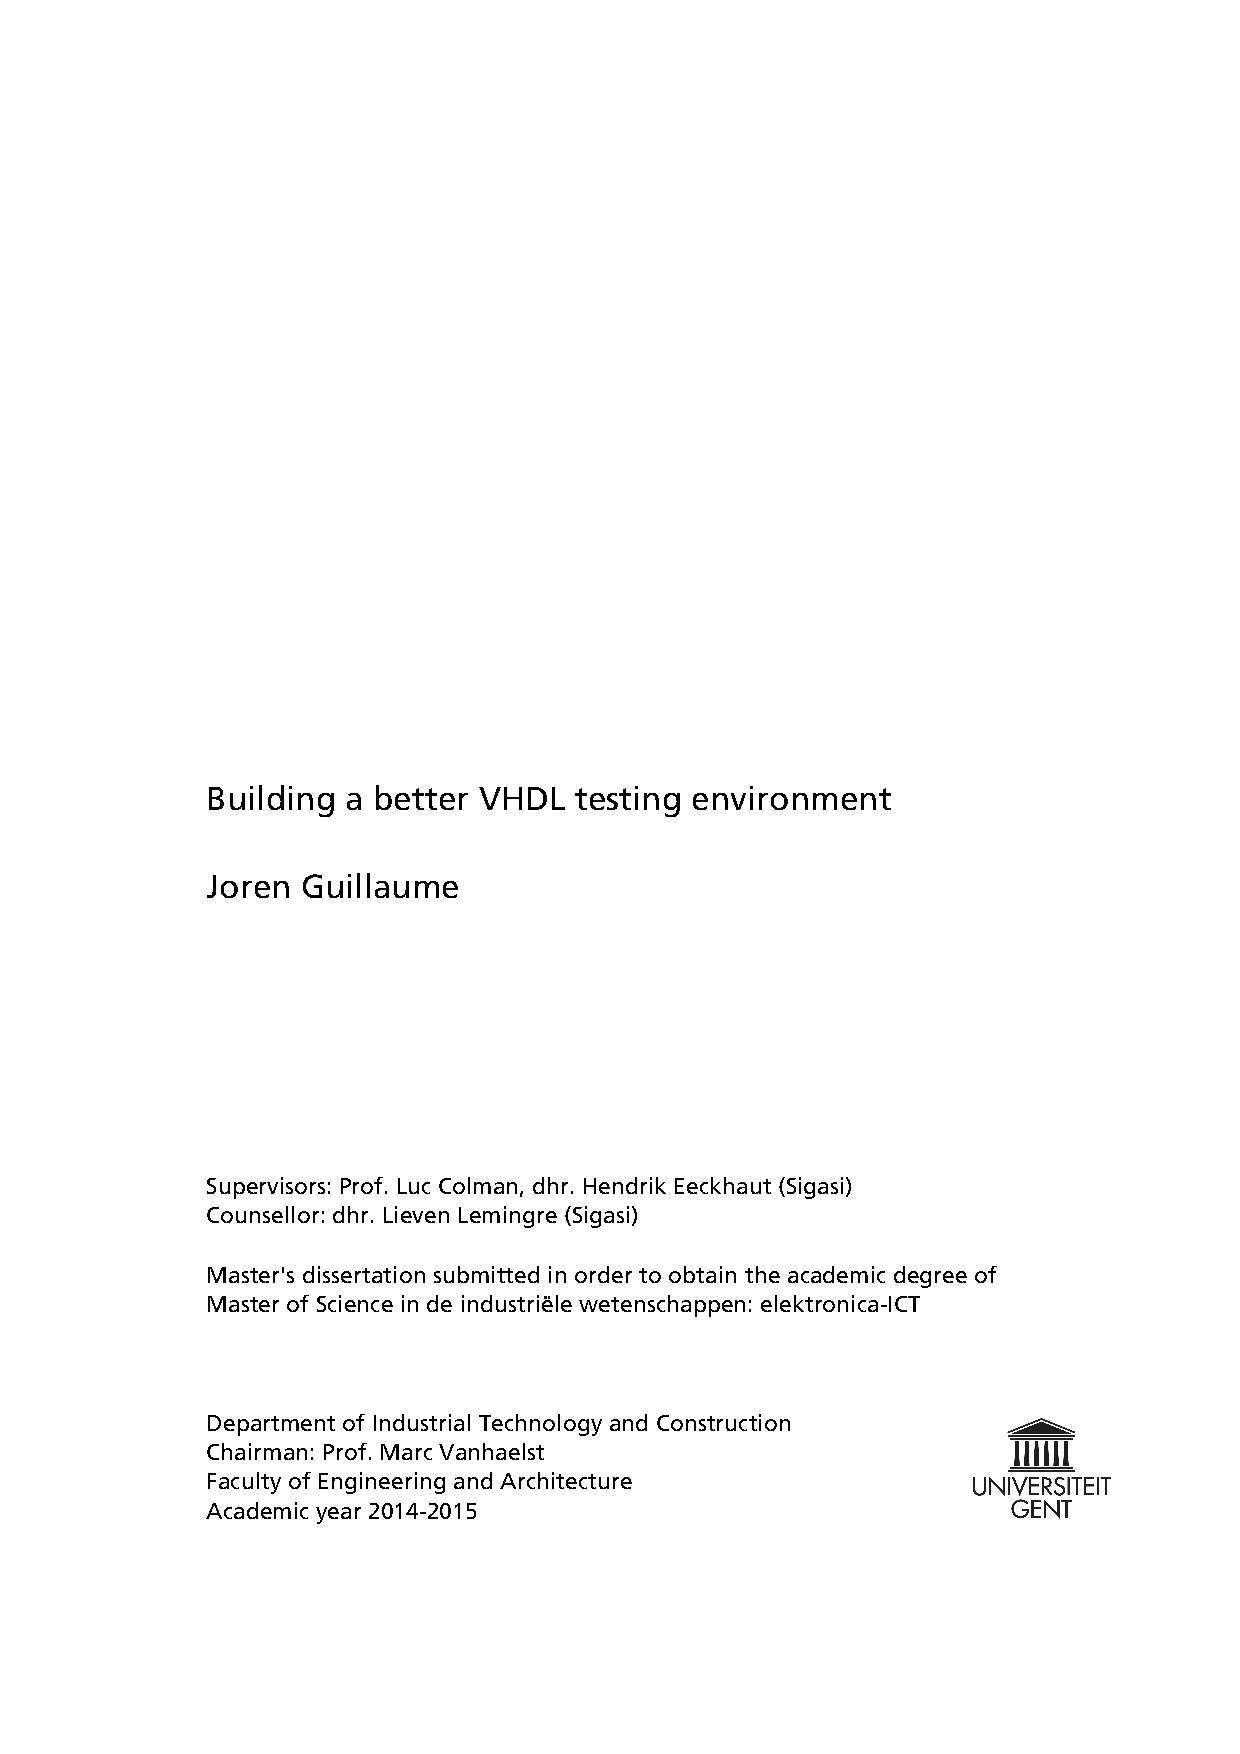
\includepdf[pages={1}]{title-generated.pdf}

%%%%%%%%%%%%%%%%%%%%%%%%%%%%%%%%%%%%%%%%%%%%%%%%%%%%%%%%%%%%
%% Copyright notice

\newpage{}
\part*{Usage restrictions}

The author gives permission to make this master dissertation available for consultation 
and to copy parts of this master dissertation for personal use. 
 In the case of any other use, the copyright terms have to be respected, in particular with regard to 
the obligation to state expressly the source when quoting results from this master dissertation.

\pagebreak{}

%%%%%%%%%%%%%%%%%%%%%%%%%%%%%%%%%%%%%%%%%%%%%%%%%%%%%%%%%%%%
%% Preface

\newpage{}\part*{Preface}
In the past year and a half I had the pleasure to work on the concept of integrating the software and hardware development worlds. In this thesis is contained the culminated knowledge and experience that was obtained during these many months, lest it be forgotten.
\\
\\
In the first part the tackled problem is explained along with a summarised background on many of the practices and concepts one needs know to fully understand the next part. In the second part the practical side of the work is demonstrated and thoughts are shared on the usability and future of this line of work.
\\
\\
\section*{Acknowledgements}
In the course of learning, producing and revising both the code and the written text many helping hands guided my way. With this I would like to extend a thanks to them.
\\
\\
To my fellow students for the pleasant atmosphere that dominated most of my studies. For providing help when asked and receiving advice without reluctance. And for those many hours spent in the telecommunications lab working side by side on many things.
\\
\\
To my supervisors prof. ir. Luc Colman and dr. ir. Hendrik Eeckhaut. The former for providing his many years of experience in supporting students, keeping a calm but firm grip on matters and always pushing to the next step. The latter for granting me the subject, providing his technical expertise and willingness to work on my problems whenever I asked.
\\
\\
Most certainly to my counsellor ir. ing. Lieven Lemiengre for providing an endless amount of feedback and brainstorming whenever. For providing technical expertise and insight when I had none to be found, for providing ideas and hooks to keep me going. For remaining realistic and setting achievable goals when the light at the end of the tunnel was darkest. And of course, for reviewing and critiquing this thesis.
\\
\\
To Jeroen Baeken and ing. Sion Verschraege for being the friends that they are. For providing feedback on anything and support whenever it was needed.
\\
\\
Finally, to my darling fianc\'{e}e Dorine Ndagsi for supporting me the many years we have been together. For providing a critical eye when needed and bringing me down a notch when explanations were overly complicated. And most certainly for being the driving force behind most of the work that got done at home, at work and in life.
\\
\\
To all those that are not named, you are not forgotten, the list would simply be endless.

\pagebreak{}

%%%%%%%%%%%%%%%%%%%%%%%%%%%%%%%%%%%%%%%%%%%%%%%%%%%%%%%%%%%%
%% Abstract

\newpage{}
\begin{abstract}
\end{abstract}

%%%%%%%%%%%%%%%%%%%%%%%%%%%%%%%%%%%%%%%%%%%%%%%%%%%%%%%%%%%%
%% Extended abstract
% Nog geen extended abstract
%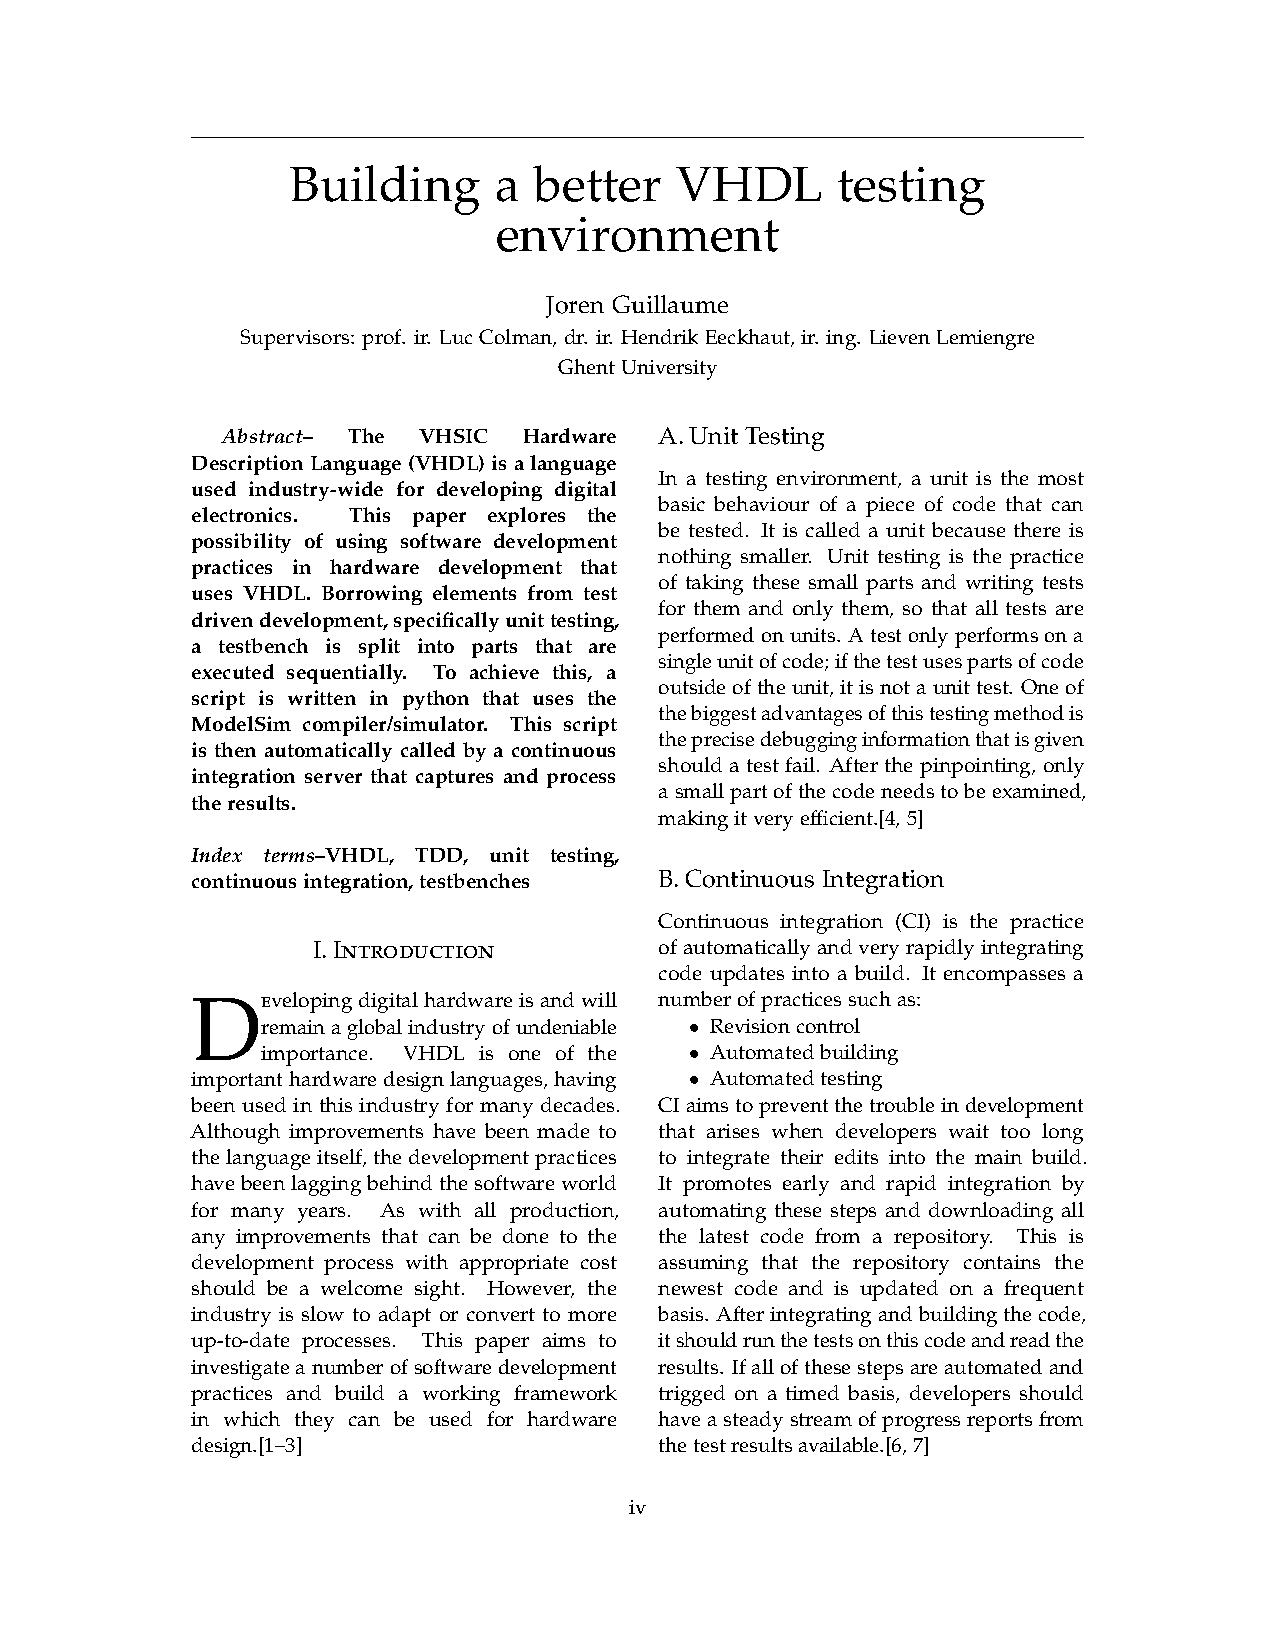
\includepdf[pages={1,2}]{extended-abstract.pdf}

%%%%%%%%%%%%%%%%%%%%%%%%%%%%%%%%%%%%%%%%%%%%%%%%%%%%%%%%%%%%
%% Table of Contents

\newpage
\setcounter{tocdepth}{2}
\tableofcontents
\pagebreak

%%%%%%%%%%%%%%%%%%%%%%%%%%%%%%%%%%%%%%%%%%%%%%%%%%%%%%%%%%%%
%% List of figures

\listoffigures
\pagebreak

%%%%%%%%%%%%%%%%%%%%%%%%%%%%%%%%%%%%%%%%%%%%%%%%%%%%%%%%%%%%
%% List of tables
% Nog geen tabellen
%\listoftables
%\pagebreak

%%%%%%%%%%%%%%%%%%%%%%%%%%%%%%%%%%%%%%%%%%%%%%%%%%%%%%%%%%%%
%% Used abbreviations and acronyms

\printglossary[type=\acronymtype,title={List of Acronyms}]
\pagebreak

%%%%%%%%%%%%%%%%%%%%%%%%%%%%%%%%%%%%%%%%%%%%%%%%%%%%%%%%%%%%
\part{Problem and background}
\renewcommand{\thepage}{\arabic{page}}
\setcounter{page}{1}

\newacronym{VHDL}{VHDL}{VHSIC Hardware Description Language}
\newacronym{VHSIC}{VHSIC}{Very High Speed Integrated Circuits}
\newacronym{TDD}{TDD}{Test Driven Development}
\newacronym{TFD}{TFD}{Test First Development}
\newacronym{CI}{CI}{Continuous Integration}

\section{Problem}
\emph{\color{red}Revisie nodig: belangrijkste pagina} \\
Developing digital hardware with the \gls{VHDL} is, like any code, prone to errors, either by the developer or by wrong product specifications. To ensure errors are weeded out before the more expensive roll-out or production begins, the code must be subjected to rigorous testing. \emph{Currently, large and impractical tests are needed to fully test a product.}
\\
\emph{\color{red}productie != einddoel alle VHDL -> FPGAs en FPGA verdelingen}
\\
\\
Because testing is such a time consuming process, finding errors often results in severe delays due to the need to both correct the error and test for others. Therefore it is in the best interests of both testing- and software engineers to write testbenches with maximal coverage, optimal readability and minimum time spent. It is also important to find and correct errors with minimal delay and maximal efficiency. This entire process should affect the least amount of code possible in order to minimize time spent retesting and modifying the code.
\emph{\color{red} Betere samenvatting + meer gevolgen}
\\
\\
In this thesis, the objective is to explore the possibility of creating an operating system independent framework. This framework should allow users to quickly and consistently create, modify, execute and evaluate testbenches. To accomplish all of this, a number of industry standard tools will be incorporated around a central Python script. This combination should ensure timely and automated building, testing and test report generation.

%\emph{\color{red}De stappen gezet, niet productie zelf}\\

\newpage{}


\section{Introduction}
\label{sec:intro}

\newacronym{CMOS}{CMOS}{Complementary Metal Oxide Semiconductor}
\newacronym{NAND}{NAND}{Not AND}
\newacronym{NOR}{NOR}{Not OR}

%\subsection{Digital Electronics}
%
%There are two kinds of electronic appliances and circuits; digital and analogue. Digital electronics differ from analogue electronics in that they use a discrete set of voltage levels to transmit signals. The most common number of items in the set is 2, a level for one (commonly
%named \emph{high}) and a level for zero (commonly named \emph{ground} or \emph{low}). The advantage of using a discrete number of levels rather than a continuous signal as is used in analogue electronics, is that noise generated by the environment, thermal noise and other interfering factors will have but a minor influence on the signal.
%\\
%\\
%To process these discrete signals, electronics are made up of transistors that nowadays are formed in with the \gls{CMOS} technology. This technology uses both an \emph{NPN} and a \emph{PNP} transistor that work in a push-pull configuration. The p's and n's in NPN and PNP simply stand for \emph{Positive} and \emph{Negative}. They are made of positively and negatively doped lumps of semiconductor, usually silicon-dioxide (SiO$_{2}$). A transistor is basically a blockage on a track and depending on the force applied to its \emph{gate}, it opens or closes the track.
%\\
%\\
%In reality, the force takes the form of a current and an NPN transistor opens its gate when a positive current is applied. A PNP transistor, however, always leaves its gate open until a current is applied. This means that if we send the same signal to an NPN and a PNP transistor, with one of the signals inverted, we can open and close two parts of the entire circuit at the same time. This is useful to both direct a certain signal to ground and at the same time close its connection with the \emph{source} (the power source). Hence also the name \emph{Complementary} MOS, the NPN and PNP complement each other.
%\\
%\\
%\newacronym{NAND}{NAND}{Not AND}
%\newacronym{NOR}{NOR}{Not OR}
%A certain combination of transistors is used to make \emph{logic gates}. These logic gates make sure that only a certain combination of ones and zeroes at the inputs result in certain ones or zeroes at the outputs. For instance, one of the most common logic gates is a \gls{NAND} gate. This gate has a number of inputs ranging from 2 to theoretically infinity (but practically 3 or 4) and only outputs a \emph{low} signal if all of the inputs are \emph{high} (digital one), otherwise its output is \emph{at ground} or \emph{low} (digital zero). The other most common logic gate is the \gls{NOR} gate. This gate outputs a low signal if any of its inputs are high, otherwise it outputs a low.
%\\
%\\
%A common mistake is to think that low or ground mean \emph{zero voltage.} This is only partially true, the high signals are measured with ground as their reference. So a high signal of 1.8 V would be 1.8 V higher than ground, and could be considered to be at 1.8 V if ground is the theoretical zero. These logic gates are themselves combined to build higher-level blocks such as flip-flops, which are used to make registers and so on up to the entire chip design.
%
%\pagebreak

\subsection{Hardware Description Languages}
\label{subsec:HDL}
\newacronym{HDL}{HDL}{Hardware Description Language}
\newacronym{RTL}{RTL}{Register Transfer Level}
A \gls{HDL} can be used to describe digital electronics, i.e. hardware, in different levels. The level that uses certain blocks of logic gates to describe more complex behaviour is called the \gls{RTL}. Some blocks are standard implementations that have been widely used and are nearly fully optimized, such as memories, flip-flops and clocks. \gls{VHDL} is such a language, having been developed in the eighties of the twentieth century, originally to have a uniform description of hardware brought in by external vendors to the U.S. department of defence. It was quickly realized that simulation was possible with a correct description and the language evolved to be used as such.\cite{vhdlorigin,vhdlorigin2} The final step was to create tools that could not only simulate, but also synthesize (i.e. create actual hardware layouts) from these descriptions.\cite{vhdlsim, vhdlsynth, vhdlsynth2, vhdlsynth3} An \gls{RTL} flip-flop implementation written in \gls{VHDL} is shown here: 
\begin{lstlisting}[language=VHDL, tabsize=4, frame=single, framesep=2mm, belowskip=16pt, aboveskip=16pt, showstringspaces=false, basicstyle=\footnotesize]
LIBRARY IEEE;
USE IEEE.std_logic_1164.ALL;

ENTITY dff IS
	PORT(d 	 : IN  std_logic;
		 clk : IN  std_logic;
		 q 	 : OUT std_logic;
END dff;

ARCHITECTURE Behavioural OF dff IS
BEGIN
	PROCESS (clk)
	BEGIN
		IF rising_edge(clk) THEN
			q <= d;
		END IF;
	END PROCESS;
END Behavioural;
\end{lstlisting}
\newacronym{IEEE}{IEEE}{Institute of Electrical and Electronics Engineers}
\newacronym{DFF}{DFF}{D Flip-Flop}
The \gls{IEEE} 1164 library provides a number of extensions on the original \gls{VHDL} IEEE 1076 specification that allow a more realistic simulation and description of hardware behaviour.\cite{IEEE1164} An \emph{entity} defines the inputs and outputs of a certain building block, in this case the \gls{DFF}. The \emph{architecture}, in this case named \emph{Behavioural}, takes the description of an entity and assigns a real implementation to it. In this architecture, we have one process and it is \emph{sequential}, meaning that every update in the process follows an update of \emph{clk}, a clock signal. The d stands for delay, and it simply puts on its output \emph{q}, that which was on the input \emph{d}, one clock period earlier. All processes are executed in parallel, this does not mean that all are triggered at the same time, nor do they take equally as long to finish, but it means that any process can be executed alongside any other process. In this case there is only one (nameless) process that describes the entire behaviour of the flip-flop. The process waits for the rising edge of the clock, which is a transition from zero to one, after which it schedules the value of d to be put on q until the next rising edge appears.
\\
\\
\newacronym{UUT}{UUT}{Unit Under Test}
\newacronym{DUT}{DUT}{Device Under Test}
This is a basic example of an entity, an architecture and a process. Before the code can be put to use in a working environment, it needs to be tested first. This is done through the use of \emph{testbenches}.\cite{bergeron00} Testbenches are made up of code that takes a certain building block, the \gls{UUT} or \gls{DUT}. The specialized tools mentioned above take the testbenches and read them. Inside are usually instructions to put a certain sequence of values on the inputs and monitor the outputs.\cite{vhdltestbench} Applying this to the example listed earlier, the testbench would contain a process with a clock, signals coupled with the ones in the entity, some stimuli and \emph{wait} statements. The signals are linked to the DFF, which is now the UUT. Then the clock starts ticking and the input d is made '0' or '1' every now and then. All that is left is to assure the output q is always '0' and '1' exactly one clock cycle later. The full code is listed in appendix~\ref{app:dfftestbench}.
\\
\\
If the device performs normally, the received output sequence should match an expected output sequence. In these testbenches it is good practice to observe how well a device performs if its inputs behave outside of the normal mode of operation. When all of these tests have finished and the output performs as expected, the device is ready to be moved further down the developmental process.\cite{vhdldebug}
\\
\\
The higher level components, such as a registry, employ a number of the lower level ones to create more complex logic.\cite{vhdlsynth3} The flip-flop could be used in certain numbers to build a \emph{register}, a collection of ones and zeroes (henceforth referred to as \emph{bits}) that is used to (temporarily) store these values. The register could then be used alongside combinational logic to build an even bigger entity. The idea here is that small building blocks can be combined to produce vast and complex circuits that are nearly impossible to describe in one go.\cite{vhdlhierarchy} Adding all these layers together also creates a lot of room for error, and having a multi-level design makes it challenging to pinpoint the exact level and location of any errors. If a device is not tested properly and faults propagate throughout development, they can be very expensive to correct.\cite{weber06} Therefore a large portion of time is spent writing and executing tests. 

%In figure~\ref{fig:Design_Flow} an overview of \gls{VHDL} design flow is given up until synthesis.
%\begin{figure}[h]
%    \centering
%	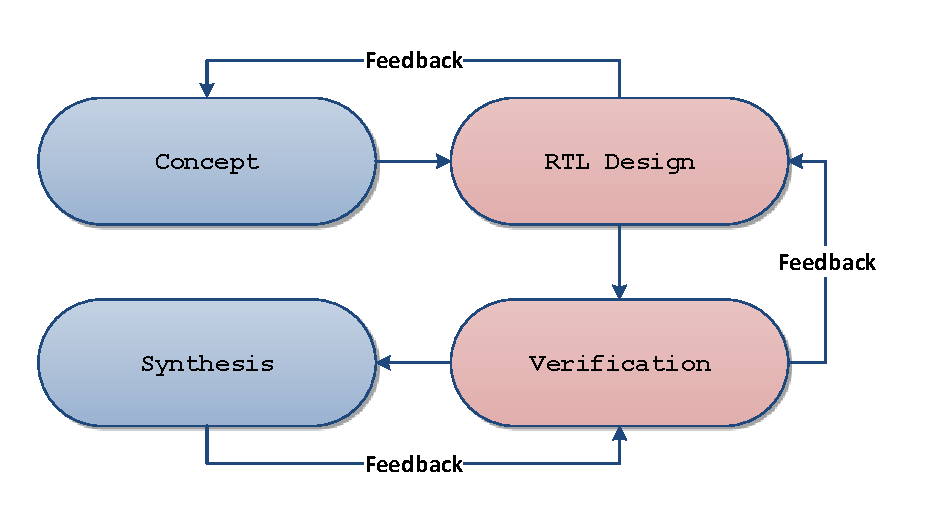
\includegraphics[width=.7\textwidth]{images/designflow.pdf}
%    \caption{Typical design flow, red indicates the main focus of this thesis.}
%    \label{fig:Design_Flow}
%\end{figure}

\newpage

%Wat zijn de gangbare praktijken in de industrie?
\newacronym{CRV}{CRV}{Constrained Random Verification}
\newacronym{DT}{DT}{Directed Testing}
\newacronym{FC}{FC}{Functional Coverage}
\newacronym{CC}{CC}{Code Coverage}
\newacronym{IC}{IC}{Intelligent Coverage}
\section{Current industry practices}
\label{sec:industry}
A number of practices exist to improve speed and quality of testing and coding. Many of these practices are already applied in the software development industry, where this is quite literally their entire business. Moving to \gls{HDL}s, it stands to reason that code meant for synthesis may not be able to follow all of these practices. However, the industry has formed several practices of its own to try and create a uniform verification process. The most well-known will be discussed in some detail below.

\subsection{Assertions}
\label{subsec:assertions}
Assertions are the standard practice of verification. An assert in VHDL is very simple: check whether some boolean condition is true.\cite{assertformal} If true do nothing, if false return the error message and throw an error of a certain level, as in the following example:
\begin{lstlisting}[language=VHDL, tabsize=4, frame=single, framesep=3mm, belowskip=8pt, aboveskip=8pt, showstringspaces=false, basicstyle=\small, linewidth=\textwidth]
assert (not Q) report "Unexpected output value" severity failure;
\end{lstlisting}
In this example, an error is thrown of the severity \emph{failure}, which ends the simulation, if the value on the output \emph{Q} (see section~\ref{subsec:HDL})) isn't \emph{logically} true. In this case it means the output has to have a value of \emph{high} or \emph{1}. The severity of the assertion can be in the range of notice to failure, and the simulator might be set to respond or stop only to a certain level of severity. Doing this for the right values at intervals gives the developer a quick overview of whether everything went according to plan. After all, if things went wrong, the assertion should have thrown an error here or there.

\subsection{The generic testbench}
The generic testbench operates as mentioned in section~\ref{subsec:HDL}. It assigns every input and output on the \gls{DUT} their counterpart in the testbench and contains a number of processes with stimuli.\cite{generictestbench} Standard procedure is:
\begin{enumerate}%[itemsep=-0.1cm]
\item Wait for some clock periods to 'ready' the design
\item Apply stimuli to the inputs
\item Wait for the appropriate number of clock cycles
\item Use asserts to check whether the outputs have the right values
\item Repeat steps 2 through 4 until satisfied
\item End with an infinite 'wait' to suspend the process
\end{enumerate}
Creating this kind of testbench for a large, hierarchical project would certainly become lengthy and unclear. To counter these disadvantages, a number of practices were created to keep control over what and how designs are tested. The more used of these practices are explained below.

\subsection{Coverage}
Coverage is a generic term that is used to describe how fully a design has been tested on one aspect or another. There exist many tools for different coverage analyses, but in this section we will focus only on the types of coverage.

\subsubsection{Code Coverage}
\newacronym{FSM}{FSM}{Finite State Machine}
In development, \gls{CC} is a type of measurement to indicate how well the source code has been tested. With the use of a coverage report, unused blocks of code can be uncovered, these blocks might indicate unnecessary code or a bug. Imagine a \gls{FSM} with an unused reset state, this might indicate that the reset isn't functioning properly or there are no tests covering the reset. However, CC does not provide any real functional analysis. It does not indicate any missing lines of code nor does it tell you whether the inputs and outputs behave properly.\cite{coverage1,coverage2}

\subsubsection{Functional Coverage}
%\emph{\color{red}Controleren}\\
\gls{FC} is the practice of measuring whether the \gls{UUT} meets with certain specifications at specific times during the testing process. These specifications are created by the developer and are used to check whether the design performs as expected. Good practice is to include corner cases, cases that cover very rare occurrences and so on. That way, the device is sure to be in working condition even under unexpected circumstances. As such, FC provides the type of coverage CC lacks.\cite{functional1,functional2}

\subsection{Verification}
\subsubsection{Constrained Random Verification}
\gls{CRV} is an industry practice where one or more inputs are generated randomly, within certain bounds or \emph{constraints}.\cite{crv1,crv2} The output is then accepted as correct if it too is within certain (other) constraints. This practice was brought into use after designs grew too large for \gls{DT} to support. DT has verification engineers write out very specific things they want to test, for instance, a reset pulse to verify the reset working correctly. CRV opposes this with the idea that for all behaviour to be tested properly in large designs, the amount of time spent writing and executing tests would simply become too great. It proposes a solution where inputs are generated randomly, within certain bounds, but in a sufficiently large quantity to have implicitly covered all scenarios. It is important to note that in DT, expected behaviour is directly tested, but in CRV it is likely to be the unexpected behaviour that gets tested too. This solved the long standing problem of testing any behaviour, including the unexpected.

\subsubsection{Formal Verification}
On top of the aforementioned, there are several more practices that have unique ways of verifying the properties of a design, but aren't used sufficiently to merit full detailing. Formal verification is such a practice, where the core idea is to mathematically prove the design from its specifications.\cite{assertformal,formal} The upside is that the design is completely verified, however, it is out of use because proving large designs is not only tedious but takes up large amounts of man-hours.

%\subsection{Methodologies}
%\emph{\color{red}Beetje overbodig of meer uitleg}\\
%\subsection{Open Source VHDL Verification Methodology}
%\newacronym{OSVVM}{OSVVM}{Open Source VHDL Verification Methodology}
%The \gls{OSVVM} is a set of packages that makes it easier for \gls{CRV} and \gls{FC} to be implemented in a project. It consists out of two packages, \emph{Random.pkg} and \emph{Coverage.pkg}. The new feature, which it dubs \gls{IC}, redefines its FC model based on holes in the FC coverage and randomization. The advantage is obviously that 100\% coverage is always within reach, even when the original draft did not achieve full coverage.\cite{ICoverage}

%\subsubsection{Universal VHDL Verification Methodology}
%\newacronym{UVVM}{UVVM}{Universal VHDL Verification Methodology}
%\emph{\color{red} To be written!}
%The Universal Verification Methodology is a popular methodology for SystemVerilog which brings it a %certain degree of automation. It should bring easier design of testing frameworks to Verilog %developers. \gls{UVVM}, however, is an intended port of features from this methodology which could be %used in VHDL verification. 

\subsection{Simulation tools}
\label{subsec:simtool}
As mentioned in section~\ref{sec:intro}, \gls{HDL}s are used for developing hardware, and need to be tested and build as such. Like many other programming language, they need a dedicated compiler to fault-check the code and build the binaries. Unlike those other programming languages they need a simulator in order to verify the builds. There exist many compilers and simulators, almost none are exclusive for \gls{VHDL}, almost all are dual-language and support some form of Verilog, a different HDL. However, many of them refuse to support the latest additions to the VHDL language specification, even the 2002 additions are hard to be found.\cite{ActiveHDL,Cadence,ISE,Quartus}

\subsubsection{ModelSim}
ModelSim is the simulator that was investigated for several reasons. Firstly, a free student edition was available. Considering licenses  outside of the educational system can easily cost upward of \$25,000 (\euro20,250 at time of writing) this made it ideal for any thesis or student related work. Proof of this is the extensive use of ModelSim in the courses related to HDL development. Secondly, ModelSim supports all versions of \gls{VHDL}, which is the \gls{HDL} we are processing. Even in 2014, only one other tool was found to support all of VHDL-2008, which is Aldec's \emph{Active-HDL}. And last but not least, ModelSim is one of the industry's most used simulators, enabling a pool of experience to be consulted.\cite{ModelSim}


\newpage{}
\section{Software development practices}
During the making of this thesis, a number of approaches were investigated and some were put to practical use. In this chapter, the more useful and tried of the aforementioned are discussed in detail.


\subsection{Test Driven Development}
\label{subsec:TDD}
\gls{TDD} is a proven development technique that has regained traction in the past decade, primarily through the efforts of Kent Beck.\cite{VHDLUnit,agiletdd} This practice has proven to increase test coverage , decrease defect density \cite{TDDinpractice} as well as improve code quality.\cite{TDDinpractice,Siniaalto,BhatN06} The technique focuses on tests being created before the actual code. It is important to make certain distinctions before going more in depth on the used methods. The developing community has a great many practices, each with their own names and methods, and hardly none are mutually exclusive.

\subsubsection{Unit testing}
To understand \gls{TDD}, a basic knowledge of \emph{unit testing} is required. In software testing, a unit test is a test designed to check a unit of code.\cite{extremeunit,VHDLunit} Ideally, this unit is the smallest piece in which the code can be divided. A unit test should always test only a single entity, and only one aspect of that entity's behaviour. This division in units has a number of benefits, one of the most important being that code is exceedingly easy to maintain. Furthermore, the division of the code makes changes, when needed, fast to be carried out and ensures that only the modified code needs to re-tested.

%% herschrijven!
\subsubsection{Test First Development}
Another main component of \gls{TDD} is \gls{TFD}, a technique that has a developer writing tests first, before any code has been written.\cite{extremeunit} This method puts behaviour as the primary drive for development. After all, if the test is conceived before the code it tests, the goal is to make the tests pass by implementing the behaviour it tests. This has developers think about what the code should do rather than what the exact implementation has to be. A key feature of a new test is that it has to fail during its first run. If not, the test is obsolete seeing as the functionality it tests has already been implemented. After being run for the first time (and failing), the developer implements just enough code to get the test to pass. Once the test succeeds, it is time for a new test.

\subsubsection{Refactoring}
The third pillar of TDD is refactoring. After the tests succeed, it is necessary to clean up the code.\cite{refactoring} A well-done \gls{TFD} implementation uses the bare amount of code needed to make the test pass, but this might not be the best code possible. Refactoring means that you take existing code and modify it to perform better. This should leave both the input and output of the tests and code unchanged, only the way the code processes input is altered. It is important in this step to edit nothing in the test code or the outputs or inputs. Otherwise, either the test would behave differently or new tests would have to be written. 

\subsubsection{Test Driven Development}
Test Driven Development is a combination of the previously mentioned techniques. A Unit Test is written before any code is, the test is then executed and should fail. After the failure, the most basic code to make the test pass is implemented. The test is then executed again and should pass. After this first pass, the code written for the passing of the test, and only this code, is edited to perform better and be less complex. This follows all steps mentioned above, a \emph{Unit Test} is written according to \emph{Test First Development} and is \emph{Refactored} later.

\begin{figure}[h]
    \centering
	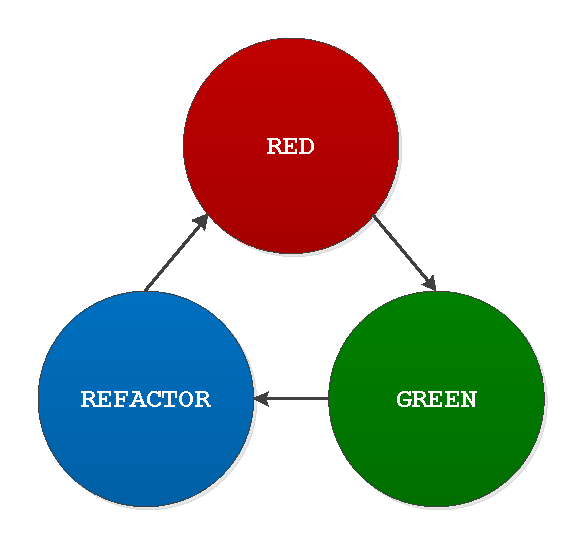
\includegraphics[width=0.38\textwidth]{images/tdd.pdf}
    \caption{Three step TDD design flow}
    \label{fig:TDD_Flow}
\end{figure}

\subsection{Continuous Integration}
\label{subsec:CI}
\gls{CI} is a software development technique in which developers upload the edits on the software, or their \emph{build}, to a central server which then \emph{continuously integrates} the code, usually from multiple developers. This to prevent integration headaches when the code of several simultaneous changes has diverged to such an extent that it would take much more time to make the edits work together than when they had been integrated early on.

\subsubsection{Revision Control}
\newacronym{RC}{RC}{Revision Control}
There are many aspects to a properly maintained \gls{CI} system, but one key aspect of overall programming has to be \gls{RC}. Not to be confused with the "undo" button in your preferred editor, a good \gls{RC} system does allow for any and all mistakes made over different edits to be undone with very little work. There exist many systems for revision control, but they all have in common that they track changes one way or the other, and most importantly that these changes can be undone. 

\subsubsection{Build Automation}
A different aspect is build automation. Using a timer or trigger, the build automatically runs with the latest updates, preferably from an \gls{RC} system. This way, the binaries are always up to date and the developer does not need to wait for compilation to run the latest tests. Although the latter is less important in a proper \gls{CI} system as will be discussed further on. 

\subsubsection{Test Automation}
As the code is built at scheduled times, and testing is needed regardless, it makes perfect sense to add a testing step to the automated build. Automating tests saves the developers yet another part of their time, thus freeing more for the actual development and debugging steps. A good \gls{CI} system can read test results and reports and preferably visualise them in a way that makes them easy to read and locate faults.
\\
\\
Combining all of these practices saves developers, and by extension the company they might work for, a lot of time and of money. Considering today's competitive market for software development, any edge that can be obtained is a plus. Even more so when plenty of free Continuous Integration solutions exist that employ open or widely used standards.\cite{ci1,ci2,ci3}

\subsection{xUnit}
\label{subsec:xUnit}
\newacronym{XML}{XML}{eXtensible Markup Language}
xUnit is a collection of frameworks that all follow the same basic principle. Its specification defines several key components for a testing framework. They encompass an implementation of a \emph{testcase} which contains a single unit test. These testcases are then enveloped in \emph{testsuites}, which are groups of tests that need the same conditions before they can be executed.  There are more implementation details but these will not be discussed.\cite{xunit2}
\\
\\
JUnit is an implementation for the Java programming language of the xUnit specification. A useful part of the specification is a standard format for the test reports. The reports are written in \gls{XML}, which is a type of language used for formatting data. The JUnit format is supported by numerous (open source) tools, which makes it an ideal candidate for further investigation.\cite{xunit,junitxml,junit}

\subsection{Python}
Python is a high-level computer programming language that first appeared in 1991, with the third major revision being released in 2008. It supports object-oriented and structured programming and is easy to use as a scripting language. A great feat of Pythons community is that there are many (open source) libraries available for just about any function that comes to mind. This on top of the already impressive amount of libraries that Python itself supports. In addition to this, Python has all of its standard features explained in great detail with good examples in its online documenting system. The combination of these features allows any programmer, even with very little know-how, to quickly put together anything that comes to mind.\cite{python1}

%Kan VHDL gemakkelijk ontwikkeld worden met Continuous Integration?
%Wat is ModelSim, waarom gebruiken? Mogelijke opties/voordelen? gratis studentenversie
%Wat is BitVis? Hoe helpt dit? 
%Wat is het marktaandeel van VHDL?
%Wat doet VHDL bij een testbench? Specialiteitjes waar er op gelet moet worden?
%Wat is de gemiddelde looptijd van een groot project?

\newpage
%\setcounter{section}{0}
\part{Developing a framework}
%\emph{\color{red}Meer grafische uitleg, workflow en dergelijke}\\
In part I different aspects from both the software and \gls{VHDL} development worlds were discussed in  varying levels of detail. In this part it is explained how bits and pieces of each subject were combined to form a new whole, a VHDL development framework.

\section{Outlining}
\label{sec:outlining}
\newacronym{OS}{OS}{Operating System}
Before work began on developing the framework, there needed to be some boundaries set and goals to work towards. As VHDL development is done on both Windows and Linux, it made sense to keep the whole framework as platform independent as possible. To add to this, the framework needsed to be developed in the short span of under a year by one developer who had little experience doing so. The language chosen thus had to be easy to master and work on all platforms with as few as possible modifications.

\subsection{First draft}
\label{subsec:first}
In section~\ref{sec:industry} some current industry practices were discussed and one of the very basic VHDL testing methods was found to be assertions. In order to remain as broad as possible, work started with processing these assertions first. As mentioned in section~\ref{subsec:TDD}, unit testing is a method that tests an as small as can be part of a code's behaviour. Applied to \gls{VHDL}, a unit test would then be the part of the code that the assertion checks. This under the assumption that the assertion checks for simple boolean truths such as \emph{output q equals '1'} and not a complex mix of logic.
\\
\\
To the likeness of unit testing, these parts of code were separated into their own testbenches. Methods of separation were not available, and thus one was developed. For complete accuracy, a lexical analyzer for VHDL would have been needed, but the development of such was worth its own thesis and as such a more simple method was used. Instead, estimation of the level of depth in the testbench structure was made using VHDL keywords such as \emph{process} and \emph{begin}.
\\
\\
Furthermore, because lexical analysis was out of the question, the constructs that each assert relied on were unable to be identified. A solution was found in the form of procedures and functions. These were placed in the architecture header, and with these single-line unit test could be called from the architecture body. All that was left for the parser to do was to find the location of these lines and place each of them in a newly created testbench.

\subsection{Draft review}
\label{subsec:review}
Even though it sounds simple, this method was still needlessly complicated and a better method had to be devised. Even then, the parser created a heap of little, seperate testbenches which added more work for the developer as he had to execute all of these separately. A possible solution was the automatic execution and result capture of the created testbenches, reducing the amount of work to a lightly modified testbench and a single execution of the parser.

\subsection{Fresh start}
As everything up until now was based on code created on the fly, it became clear that the original files weren't ready to be refactored or otherwise modified. The experience gained from writing everything mentioned in section~\ref{sec:outlining} was put to good use, and a clean build was started. With this build a number of assumptions were made:
\begin{itemize}
\item Optional arguments to modify the behaviour should be specified
\item Full on automation should be included
\item A log detailing events should be held
\item Proper documentation should be provided
\end{itemize}
All of these modifications made the framework more suitable for developers. The optional arguments would allow for a greater control over the program. The automation countered the extra work created from the generation of all the separate testbenches. The log made it easier to figure out where things went wrong should they go wrong. And lastly, the documentation was a given for any decent project.

\newpage{}
\section{Using the framework}
\label{sec:using}
For the framework to be properly usable, a number of things had to be considered. Firstly, not all testbenches were suited to be processed by the parser; it relied heavily on the independence of tests from one another. Therefore, tests that relied on outputs from previous tests needed to be kept together, which lead to a large portion of such testbenches needing to be completely rewritten.
\\
\\
Secondly, even with properly suited testbenches, the output needed to remain uniform and recognizable. As mentioned in section~\ref{subsec:first}, to have this done automatically would have required a full blown lexical analysis which was simply too complex. As a solution, the use of a testing library was proposed which would provide uniform tests and output.

\subsection{Preparing the testbench}
\label{subsec:preparing}
For the testbench to be properly parsed, it needed some preparation first. The blocks of tests, henceforth referred to as testsuites, were to be independent and separated by keywords that signify the beginning and end of a testsuite. Not only this, but the standard asserts were to be replaced with functions from the library, and the library of course needed to be included. An example using the \gls{DFF} from section~\ref{subsec:HDL} (full code in appendix~\ref{app:dfftestbench}):
\begin{lstlisting}[language=VHDL, tabsize=4, frame=single, framesep=2mm, belowskip=8pt, aboveskip=8pt, showstringspaces=false, basicstyle=\footnotesize]
	...
		assert q = '0'
			report "Wrong output value at startup" severity FAILURE;
		d <= '1';
     	WAIT FOR clk_period;
     	assert q = '1'
			report "Wrong output value at first test" severity FAILURE;
	...
\end{lstlisting}
Would turn into (See appendix~\ref{app:dfftestbench2}):
\begin{lstlisting}[language=VHDL, tabsize=4, frame=single, framesep=2mm, belowskip=8pt, aboveskip=8pt, showstringspaces=false, basicstyle=\footnotesize]
	...
		--Test 1
		check_value(q = '0', FAILURE, "Wrong output value at startup");
		write(d, '1', "DFF");
		check_value(q = '1', FAILURE, "Wrong output value at first test");
		...
		--End 1
	...
\end{lstlisting}
In the full code it is shown that the functions are overloads of existing functions in the \emph{BitVis} library, which will be discussed in section~\ref{subsec:bitvis}. Also visible here are the keywords \emph{-\--Test} and \emph{-\--End} with which the testsuites are separated. The number next to it is a testsuite identifier, but was not necessary as the parser kept track of the count.
\\
\\
Overloading functions, using libraries and seemingly completely overhauling the testbench may appear to be like a lot of work for a small testbench such as this. While true, this method was easily scalable for testbenches of much larger sizes and with designs of greater complexity. If the developer created a testbench starting with this approach, no time would have been wasted redoing any code and the readability would have been greatly improved. Lastly, automated logging was built in these procedures to keep track of progress during testruns. This allowed for easier and uniform report generation (see section~\ref{subsec:reports}).

\subsection{Calling the parser}
\label{subsec:parser}
The parser was created as a script, written in Python, thus it was necessary to have access to a command-line interface as python requires one to run its scripts. Originally, using the parser was as easy as typing \emph{python testbench\_parser.py tb\_dff.vhd} in the command-line. There was one testbench to be parsed and everything happened automatically according to default methods, hardcoded in the script. During further development it became clear that there were many ways a developer might want to test their project. As such there was a need for a way to modify the parser's behaviour when it ran. Possible solutions included different scripts, a settings file but ultimately the decided upon method was the use of arguments.

\subsubsection{Arguments to the parser}
\label{subsec:argparser}
Python had a built-in argument parser, in the library \emph{argparse}. With this it became possible to have a complex yet simple to use command-line interface with both optional and required arguments. Included in the library was the option for a clear and thorough help, providing users with all the information they needed to run the script. A simple example is listed below:
\begin{lstlisting}[language=bash, tabsize=4, frame=single, framesep=2mm, belowskip=8pt, aboveskip=8pt, showstringspaces=false, basicstyle=\footnotesize]
$ python src\testbench_parser.py -m partitioned -l  Project\sim\tb_dff_r.vhd -c
\end{lstlisting}
By using this command, the testbench from appendix~\ref{app:dfftestbench2} was processed using the \emph{partitioned} method, which is the method that uses the keywords \emph{Test} and \emph{End} (see section~\ref{subsubsec:processmethods}). The \emph{-c} flag ensured that output of the simulator (in this case ModelSim) was displayed and not just captured and stored as was default. Below are all the flags and their help text:
\begin{itemize}[itemsep=-.05cm]
\item \itab{'-c', '-\--cmd'} \tab{specifies output to be displayed on the command line}
\item \itab{'-d', '-\--dest'} \tab{specifies a custom path for the log}
\item \itab{'-f', '-\--file'} \tab{specifies -l/-\--list is a file with a list of .vhd files}
\item \itab{'-l', '-\--list'} \tab{specifies the list of .vhd files to be processed (at least one)}
\item \itab{'-m', '-\--method'} \tab{specifies what method was used to write the testbench}
\item \itab{'-p', '-\--precompiled'} \tab{specifies location of the precompiled dependencies, requires full path}
\item \itab{'-r', '-\--runops'} \tab{specifies custom arguments for simulation start}
\item \itab{'-v', '-\--version'} \tab{specifies a different VHDL version, default is 2008}
\end{itemize}
With this parser, it also became possible to run multiple testbenches with one call to the script. This allowed to test multiple levels of a hierarchic design, or even completely different designs in one run. Most of the flags are self-evident, but those that are not are explained below.
\\
\\
The \emph{-p} or \emph{-\--precompiled} flag points to a text file that contains instructions very similar to those found in a unix \emph{Makefile}. They are commands that need to be executed before the testbench can be compiled. This would be all of the source files used, in their specific order and any special libraries that need to be created beforehand. A full editor might have recognized the dependencies and libraries on its own and created a Makefile or similar accordingly but here the lack of a decent lexical analysis prevented this.
\\
\\
The\emph{-r} or \emph{-\--runops} flag is to specify a custom command for ModelSim to run during the execution of the newly made testbenches. The default value is \emph{-do "run -all;exit"}, which simply starts the simulation until its end and then exits. However, developers might want to load different memory files in a memory or specifiy a custom file with more elaborate commands.

\subsubsection{Processing methods}
\label{subsubsec:processmethods}
In section~\ref{subsec:argparser} the processing method \emph{partitioned} was mentioned as well as the \emph{-m} or \emph{-\--method} flag. The parser thus supported multiple methods of dividing the testbench, they are listed below:
\begin{itemize}%[itemsep=-0.1cm]
\item Start Stop with identifiers
\item Line per line 
\item Partitioned with identifiers
\end{itemize}
In the Start Stop method, every single line between certain keywords was assumed to contain a test. It was assumed that everything above the keywords was architecture header and everything below was a general 'end of the architecture body'. This method was the easiest to parse, it looked for \emph{-\--Start} and created a new testbench with every line until \emph{-\--Stop}.
\\
\\
In the Line method, the parser looked for a process. This process should contain one test per line. It tried to identify this process on its own and as such, could easier make a mistake than the Start Stop method.
\\
\\
Finally, in the Partitioned method, the developer indicated which blocks are testsuites by using the \emph{-\--Test} and \emph{-\--End} keywords. Everything in between these keywords was assumed to be a single block of testcases, to be put in the same new testbench. As such, and unlike the previous two methods, it was possible to define multiple testsuites. 

\subsection{Report and log generation}
\label{subsec:reports}
After the parser from section~\ref{subsec:parser} had run its course, results were captured automatically. However, making sense of a whole lot of command line output from a text file was challenging. ModelSim made this more difficult by adding a header and a lot of information that isn't really interesting at that time of development. Things such as which files were loaded prior to the execution and which preference file was being read were not needed for a quick overview. However, they might have still be needed in the event of severe failure.

\subsubsection{Basic report}
A great deal of filtering of the output file was required, only the passed and failed testresults were needed for a proper report. Whether tests passed or failed was outputted with easy to recognize keywords. A simple filtering on these words per line of the output file returned every testresult, neatly ordered in passed and failed groups. A total testcount was tallied from the combination, and as such a crude report was written to a text file.

\subsubsection{XML report}
Previously discussed in section~\ref{subsec:xUnit}, the JUnit implementation of xUnit uses \gls{XML} for report viewing. The editor that was used throughout the development of the thesis is \emph{Eclipse}, which was written in Java, the same language JUnit is an implementation for. They could be read and displayed in Eclipse by manually navigating to them or editing the project properties to automatically read them.
\\
\\
To create the XML reports, a pre-made, open-source Python implementation of a JUnit report generator, aptly named python-junit-xml was used. This package required its own external component to be installed, called setuptools.\cite{junitxml, setuptools} In this thesis, versions 1.0 and 3.5.1 respectively were used, but versions 1.3 and 8.0.4 are available at time of writing. 

\subsubsection{Logkeeping}
Finally, a log was kept detailing events throughout the parser's execution. It contained critical events along with timestamps for precise debugging. Everything within this log file was related to only the parser and its workings. The file that contained details about ModelSims execution was not saved.

%Wat is CI? Wat doet Hudson?
%GIT? Hoe werkt het, waarom?
%Waarom automated? Voordelen?
%Problemen bij implementatie? Tekortkomingen?
\subsection{Hudson-CI}
\label{subsec:Hudson}
For full automation, a \gls{CI} system was integrated into the framework. The \gls{CI} solution that was incorporated was Hudson-CI which provided an extensive range of features including:
\begin{itemize}%[itemsep=-0.1cm]
\item Timed and triggered building from an \gls{RC} repository
\item Automated testing of builds
\item Reading reports in the JUnit format
\item Graphical and statistical overview of test results throughout builds
\end{itemize}
Hudson was available as a running .war file (a Java web application that runs on a local machine) or as an installed service.\cite{hudson} The version used throughout this thesis is 3.2.0 but at time of writing 3.2.1 is available.

\subsubsection{Using Hudson-CI}
For ease of use, Hudson was installed as a local service. By default it is accessed at port 8080 of the local machine, usually by typing \emph{localhost:8080} in a browser. The following steps were followed to successfully complete several testruns on a Windows 8 machine:
\begin{enumerate}
\item Create a new job with:
\begin{enumerate}
\item Git repository as SCM
\item The batch command listed in section~\ref{subsec:argparser}.
\item JUnit test results published under \emph{VHDL\_TDD\_Parser/*/*.xml}
\item Manual build activation
\end{enumerate}
\item Press the \emph{Build now} button
\end{enumerate}
This automatically downloaded the source, compiled the external testbench for the \gls{DFF}, executed the different architectures, captured and formatted the output and published the \gls{XML} report. For successive runs only step 2 had to be repeated, the code is automatically updated from git should it change. An example of captured statistics is shown in appendix~\ref{app:hudsonstats}.

\subsection{Bitvis utility library}
\label{subsec:bitvis}
Throughout the development of the framework multiple approaches were used to enhance developer experience including a library with widely used and usable functions. At first this was a self developed library, however, after a short while the existing \emph{Bitvis utility library} was used. It was developed by the Norse company Bitvis for verification and compatible with all versions of \gls{VHDL}. \cite{bitvis} The library promoted overloading its functions with implementations for the project that was being developed. It also provided an easy to use logging function with great customizability, which made it ideal for use in the framework.
\\
\\
To make use of the library, all that needed to be done was to include it in the project, use its functions and overload where needed. For the framework, the use of the \emph{check} or \emph{check\_value} function was critical seeing as the test parser relied on the output created by this function to assess test success. An example is listed below (full code in appendix~\ref{app:dfftestbench2}):
\begin{lstlisting}[language=VHDL, tabsize=4, frame=single, framesep=2mm, belowskip=8pt, aboveskip=8pt, showstringspaces=false, basicstyle=\footnotesize]
...
LIBRARY bitvis_util;
USE bitvis_util.types_pkg.ALL;
USE bitvis_util.string_methods_pkg.ALL;
USE bitvis_util.adaptations_pkg.ALL;
USE bitvis_util.methods_pkg.ALL;
	...
	PROCEDURE log(
    	msg   : STRING) IS
    BEGIN
      log(ID_SEQUENCER, msg, C_SCOPE);
    END;
    
	PROCEDURE write(
    	SIGNAL   data_target  : IN STD_LOGIC_VECTOR;
    	CONSTANT data_value   : IN STD_LOGIC_VECTOR;
    	CONSTANT msg          : IN STRING) IS
    BEGIN
    	data_target <= data_value;
    	WAIT FOR clk_period;
    	log(msg & " write(Target:" & to_string(data_value, HEX, AS_IS, INCL_RADIX) 
    		& ", " & to_string(data_target, HEX, AS_IS, INCL_RADIX) & ")";);
    END;
	...
		write(d, '1', "DFF");
		check_value(q = '1', FAILURE, "Wrong output value at first test");
	...
\end{lstlisting}


\newpage{}
\section{Future work}
While a working framework was achieved, many parts are missing for a usable whole. Below are listed some of the more critical absent pieces as well as suggestions that are not necessarily needed for a working framework but might make development more pleasant.

\subsection{Wider tool support}
In section~\ref{subsec:simtool} it was decided to support ModelSim as the compiler for the framework. Despite its extensive use in the classroom, it is not the only tool at the top. Different tools might use other methods, accept different input and produce different output. While there are too many tools to support them all, either a general approach can be achieved or the most widely used can be integrated.
\\
\\
On the topic of tools, the current support of ModelSim itself is limited at best. Only the very basic steps have been taken to assure compiling. Complex projects might need an extensive list of options to be run before compiling, during simulation or otherwise.

\subsection{Lexical analysis}
In section~\ref{sec:outlining} it was decided that lexical analysis was out of the question. However, future modification should include this as the advantages greatly outweigh the work that it requires. A full lexical analysis should allow for more advanced methods of testbench creation to be supported, as well as a precise integration for current methods. Furthermore, a good analysis could separate a testbench on its own, seeing dependencies and eliminating code duplication. And lastly, a great analysis might even be able to convert testbenches to the used methods by recognizing groups of test, make its own functions out of them and saving developers a lot of time in the process.

\subsection{Adapted CI tool}
In section~\ref{subsec:CI} continuous integration was introduced and in section~\ref{subsec:Hudson} Hudson-CI was proposed as the \gls{CI} tool. However, Hudson-CI is a software development tool meant for software development practices. Its inner workings have shortcomings that, while not life-threatening, are needed for hardware developers. The JUnit reports, for instance, do not recognize sub-millisecond times, and debugging output of the compiler could be integrated. A dedicated hardware CI tool might be developed to provide full support for all the features that are lacking.


\newpage{}
\section{Commentaries on developing VHDL}
During the making of this thesis a great deal of time was spent working with \gls{VHDL} and testbenches in particular. Evaluating, re-evaluating and dissecting these testbenches to find ways to improve their workings and their developing environment brought good familiarity with the inner workings. As such, certain aspects of the language and its surroundings or lack thereof were the proverbial thorn in the eye and could stand to be improved.

\subsection{An industry stuck in 1993}
\label{subsec:stuck}
in section~\ref{sec:industry} industry standard practices were discussed along with some considerations on the tools used in section~\ref{subsec:simtool}. While there definitely is work being done to improve the coding practices, the hardware development world is slow to adapt to any change. The biggest proof of this is that just now (Q4 2014) slow adaptations are being made for the latest VHDL standard, which was defined in 2008. The lack of willingness to improve upon working methods -"\emph{Don't fix what isn't broken.}"- stifles innovation. Luckily for the language the industry is a very niche world of behemoths that doesn't see many competitors gain much traction fast.

\subsection{Lack of reflection or introspection}
Reflection and introspection are two programming concepts, the former already existing since assembly languages were used. Reflection means that a programming language can modify parts of its innards at runtime. While this certainly sounds not synthesizable, it could bring about a revolution in the creation of functions for testbenches. Instead of having to overload for an unreasonable amount of different configurations, code would simply adapt to the situation by adjusting its arguments to the right type. This, of course, providing the function's structure  continues to work after the modifications.
\\
\\
Introspection can be seen as a part of reflection, it is the ability to examine an object at runtime. While VHDL is not an object-oriented programming language, signals, variables and constant can be seen as a type of object. They have many possible configurations and can have  properties such as vector length. Being able to examine these properties at runtime and matching object types against each other would provide for some of the same functionality mentioned with reflection.

\subsection{Hardware developers are not software developers}
While considering the previous commentaries it became clear that a major shortcoming of hardware developers is that they are not trained to develop software. Software developers learn certain practices, methods, group works and the likes in the course of their education. Hardware developers usually come from an engineering background where sciences and knowledge of \emph{what} is being developed is taught. This creates a work environment where seldom there is a developer taught in software development methods. Combined with the slow and stagnant change mentioned in section~\ref{subsec:stuck} this leads to outdated development practices.
%Wat zijn de ontbrekende features voor het geavanceerd testen van VHDL?
%Wat kan er verbeterd worden aan de VHDL specificatie?
%Hoe kunnen de programmas (compilers e.d.) aangepast worden zodat dit overkomen wordt?
%Verschil in ervaring elektronici met programmeren versus ervaring informatici met elektronica
%introspectie
%reflectie

\newpage{}
\section{Conclusion}
%Wat hebben we gedaan en hoe hebben we het bereikt? (beknopte versie)
%-> State facts
At the start of this thesis, it was stipulated that developing \gls{VHDL} is prone to errors and that the testbench and its environment play an integral part in locating and solving these. As a solution, a testing framework was proposed that would work around a central script and integrate ideas from the software development world.
\\
\\
A first draft revealed many shortcomings of the methods investigated and a subsequent revision was scheduled. More detailed outlines provided better planning and easier incorporation of the envisioned methods as well as a better coding practice.
\\
\\
The framework was made to integrate one of the most commonly used simulation tools, ModelSim. Around it, the software development practice of continuous integration was built using the Hudson-CI tool. Hudson-CI was used to retrieve the code from an RC repository, call the script and display its output.
\\
\\
The central script was made to accept different forms of modified testbenches and it was made possible to modify the behaviour of the script with command-line arguments. A full text output report, a text summary and a processed report in the JUnit XML format were made available after compilation and simulation.
\\
\\
Compilation and simulation test runs were performed with a simple example and found to be working as expected. Runs with more complicated testbenches were found to be lacking in support and not fully completing.
\\
\\
The objective of developing a framework was generally achieved, but it severely lacked in implementation details. Better support for the current tools and support for more a larger variety of tools is absolutely necessary for a working framework. Finally, it was most definitely shown that applying software development practices is possible and useful in a hardware development environment.

\pagebreak{}

\printbibliography[heading=bibintoc]

\newpage{}

\begin{appendices}

\section{Code examples}
\subsection{DFF testbench}
\label{app:dfftestbench}

\begin{lstlisting}[language=VHDL, tabsize=4, frame=single, framesep=2mm, belowskip=4pt, aboveskip=4pt, showstringspaces=false, basicstyle=\scriptsize]
LIBRARY IEEE;
USE IEEE.std_logic_1164.ALL;

ENTITY tb_dff_r IS
END tb_dff_r;

ARCHITECTURE Behavioural OF tb_dff_r IS
	COMPONENT dff
    PORT(
		d 	: IN  STD_LOGIC;
        clk : IN  STD_LOGIC;
		q 	: OUT STD_LOGIC;
    END COMPONENT;
    
	SIGNAL d   : STD_LOGIC := '0';
	SIGNAL clk : STD_LOGIC := '0';
	SIGNAL q   : STD_LOGIC := '0';

	CONSTANT clk_period : TIME := 10 ns;
	
BEGIN
	uut: dff PORT MAP (
        d 	=> d,
        clk => clk,
		q 	=> q
        );
	clk_process : PROCESS
		BEGIN
			clk <= '0';
			WAIT FOR clk_period/2;
			clk <= '1';
			WAIT FOR clk_period - clk_period/2;
	END PROCESS;
	
	stim_proc: PROCESS
	BEGIN		
     	WAIT FOR clk_period;
     	ASSERT q = '0'
			REPORT "Wrong output value at startup" SEVERITY FAILURE;
		d <= '1';
     	WAIT FOR clk_period;
     	ASSERT q = '1'
			REPORT "Wrong output value at first test" SEVERITY FAILURE;
		d <= '0';
     	WAIT FOR clk_period;
     	ASSERT q = '0'
			REPORT "Wrong output value at final test" SEVERITY FAILURE;
		WAIT;
   END PROCESS;
END Behavioural;
\end{lstlisting}

\newpage{}
\subsection{Revised DFF testbench}
\label{app:dfftestbench2}
\begin{lstlisting}[language=VHDL, tabsize=4, frame=single, framesep=2mm, belowskip=4pt, aboveskip=4pt, showstringspaces=false, basicstyle=\scriptsize]
LIBRARY IEEE;
USE IEEE.std_logic_1164.ALL;

LIBRARY bitvis_util;
USE bitvis_util.types_pkg.ALL;
USE bitvis_util.string_methods_pkg.ALL;
USE bitvis_util.adaptations_pkg.ALL;
USE bitvis_util.methods_pkg.ALL;

ENTITY tb_dff IS
END tb_dff;

ARCHITECTURE Behavioural OF tb_dff IS
	COMPONENT dff
    PORT(
		d 	: IN  STD_LOGIC;
        clk : IN  STD_LOGIC;
		q 	: OUT STD_LOGIC;
    END COMPONENT;
    
	SIGNAL d   : STD_LOGIC := '0';
	SIGNAL clk : STD_LOGIC := '0';
	SIGNAL q   : STD_LOGIC := '0';
	CONSTANT clk_period : TIME := 10 ns;
	
	PROCEDURE log(
    	msg   : STRING) IS
    BEGIN
      log(ID_SEQUENCER, msg, C_SCOPE);
    END;
    
	PROCEDURE write(
    	SIGNAL   data_target  : IN STD_LOGIC_VECTOR;
    	CONSTANT data_value   : IN STD_LOGIC_VECTOR;
    	CONSTANT msg          : IN STRING) IS
    BEGIN
    	data_target <= data_value;
    	WAIT FOR clk_period;
    	log(msg & " write(Target:" & to_string(data_value, HEX, AS_IS, INCL_RADIX) 
    		& ", " & to_string(data_target, HEX, AS_IS, INCL_RADIX) & ")";);
    END;
BEGIN
	uut: dff PORT MAP (
        d 	=> d,
        clk => clk,
		q 	=> q
        );
	clk_process : PROCESS
		BEGIN
			clk <= '0';
			WAIT FOR clk_period/2;
			clk <= '1';
			WAIT FOR clk_period - clk_period/2;
	END PROCESS;
	
	stim_proc: PROCESS
	BEGIN		
		check_value(q = '0', FAILURE, "Wrong output value at startup");
		write(d, '1', "DFF");
		check_value(q = '1', FAILURE, "Wrong output value at first test");
		write(d, '0', "DFF");
		check_value(q = '0', FAILURE, "Wrong output value at final test");
   END PROCESS;
   
END Behavioural;
\end{lstlisting}

\newpage{}
\section{Figures}
\subsection{Hudson-CI example statistics}
\label{app:hudsonstats}
\begin{figure}[h]
    \centering
	%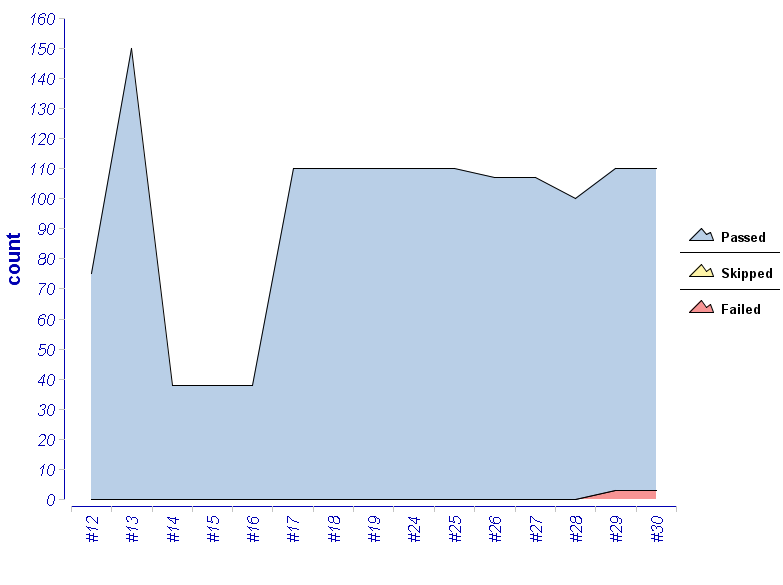
\includegraphics[width=.7\textwidth]{images/hudsonstats.png}
	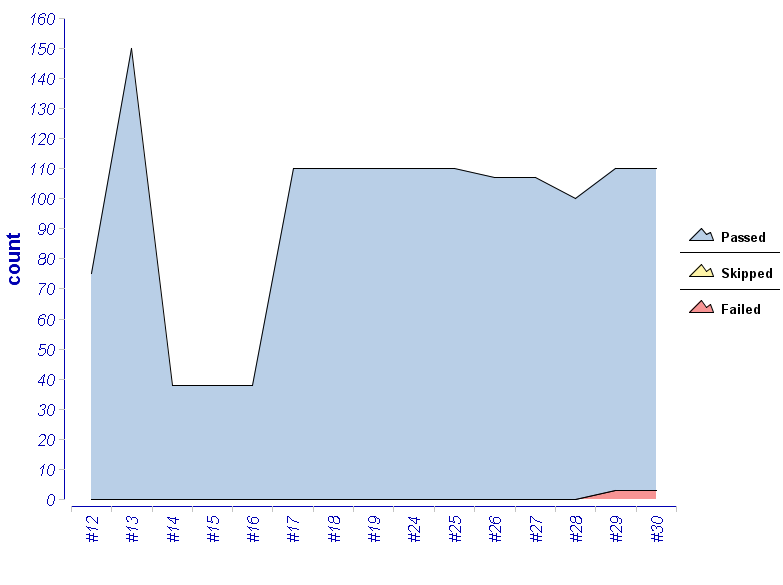
\includegraphics[width=.85\textwidth]{images/hudsonstats.png}
    \caption{Hudson-CI example statistics.}
    \label{fig:Hudson-CI example statistics}
\end{figure}

\end{appendices}

%%%%%%%%%%%%%%%%%%%%%%%%%%%%%%%%%%%%%%%%%%%%%%%%%%%%%%%%%%%%
%% 

%\newpage{}
%\begin{landscape}
%\part{Appendix}
%\section*{Code}
%\lstinputlisting[language=Python, basicstyle=\tiny]{H:/Users/Joren/Documents/GitHub/VHDL/src/%testbench_parser.py}
%\end{landscape}


%%%%%%%%%%%%%%%%%%%%%%%%%%%%%%%%%%%%%%%%%%%%%%%%%%%%%%%%%%%%
%% Mandatory blank page
\afterpage{\blankpage}


\end{document}
